\documentclass{beamer}
\usetheme{Rochester}
\usecolortheme{lily}

\usepackage{subcaption}

\title{Walk Around The World}
\subtitle{Gamification of Exercise}
\author{Ryan Wells - 1002253w}

\begin{document}
\maketitle
\begin{frame}
  \frametitle{Contributions}
  
  \begin{itemize}
    \item Comparison of gamification in exercise.
    \item ``Urban Explorer'' Android app.
    \item Two design/implementation iterations of ``Urban Explorer''.
    \item Evaluation of our gamification techniques.
  \end{itemize}
\end{frame}

\begin{frame}
  \frametitle{Gamification}
  \begin{itemize}
    \item Using games to encourage users and change behaviour. 
    \item Story, Achievements, Leaderboards and Social Interaction.
  \end{itemize}

  \begin{figure}[h]
    \centering
    \begin{subfigure}[b]{0.3\textwidth}
      
\includegraphics[width=\textwidth]{images/charity-miles.jpg}
      \caption{Charity Miles}
    \end{subfigure}
    \hspace{0.02\textwidth}
    \begin{subfigure}[b]{0.3\textwidth}
      
\includegraphics[width=\textwidth]{images/walk.png}
      \caption{WalkJogRun}
    \end{subfigure}
    \hspace{0.02\textwidth}
    \begin{subfigure}[b]{0.3\textwidth}
      
\includegraphics[width=\textwidth]{images/fitbit.png}
      \caption{Fitbit}
    \end{subfigure}
  \end{figure}  

\end{frame}

\begin{frame}
  \frametitle{Gamification}
  \begin{itemize}
  \item Play to Cure: Genes in Space.
  \item Foldit.
  \item World Without Oil.
  \item Chick Clique.
  \end{itemize}
\end{frame}

\begin{frame}
  \frametitle{Defining Gamification}
  ``The process of game-thinking and game mechanics to engage users
  and solve problems.''

  \hfill \emph{Gamification By Design}
  
  \hfill Gabe Zichermann and Christopher Cunningham
  
  \vspace{20pt}
  
  The ``Elemental Tetrad'' (\emph{The Art of Game Design}, Jesse Schell):
  \begin{itemize}
    \item Story
    \item Mechanics
    \item Aesthetics
    \item Technology
  \end{itemize}
\end{frame}

\begin{frame}
  \frametitle{Defining Gamification}
  ``The process of game-thinking and game mechanics to engage users
  and solve problems.''

  \begin{description}
    \item[Problem -] View that there is a``lack of time to take exercise''.
    \item[Users -] Do not exercise frequently but who have time in
      their daily routine that has potential to be converted to
      exercise. 
    \item[Game Mechanics -] Exercising outdoors to receive awards.
    \item[Game Thinking -] User wants success. Walking an extra five
      minutes could grant this success.
  \end{description}
\end{frame}

\begin{frame}
  \centering
  Run Around the World! 
  \frametitle{Urban Explorer}
    \begin{figure}[h]
    \centering
    \begin{subfigure}[b]{0.3\textwidth}
      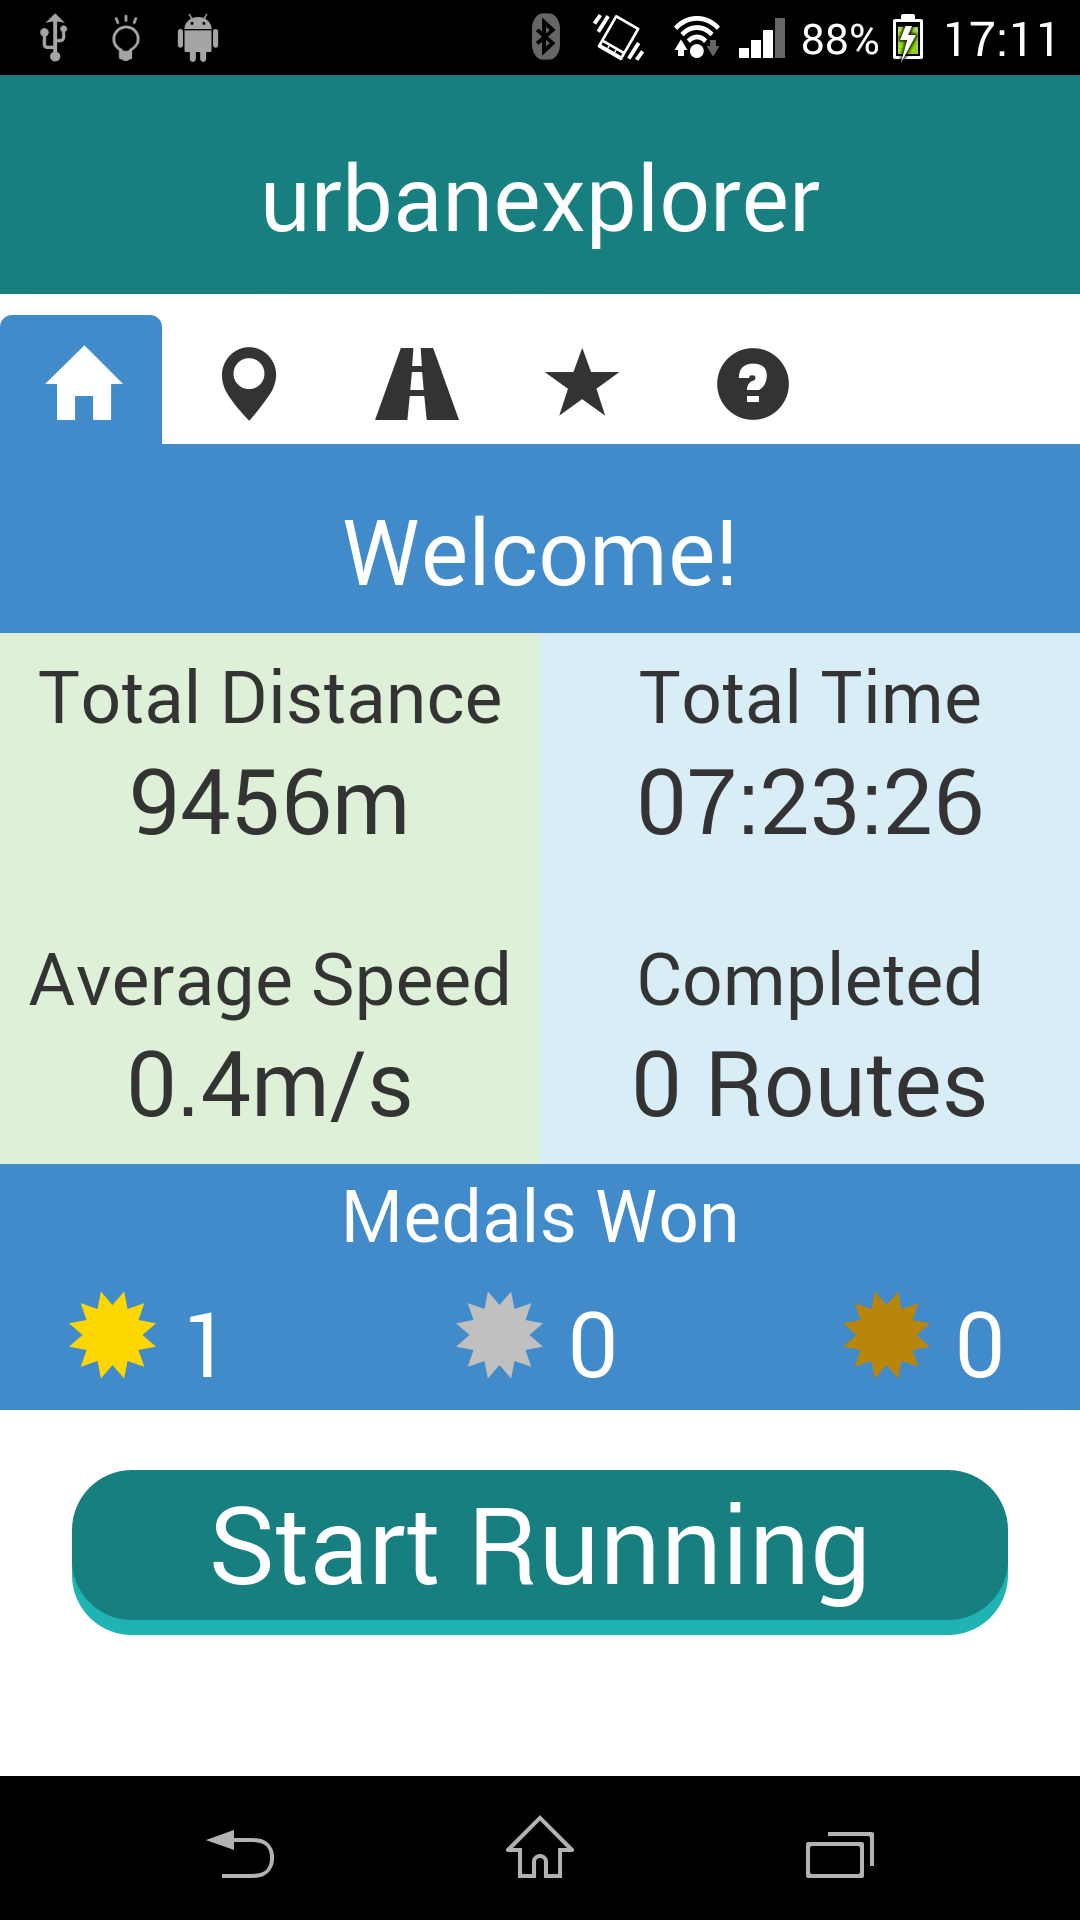
\includegraphics[width=\textwidth]{images/home.png}
    \end{subfigure}
    \hspace{0.02\textwidth}
    \begin{subfigure}[b]{0.3\textwidth}
      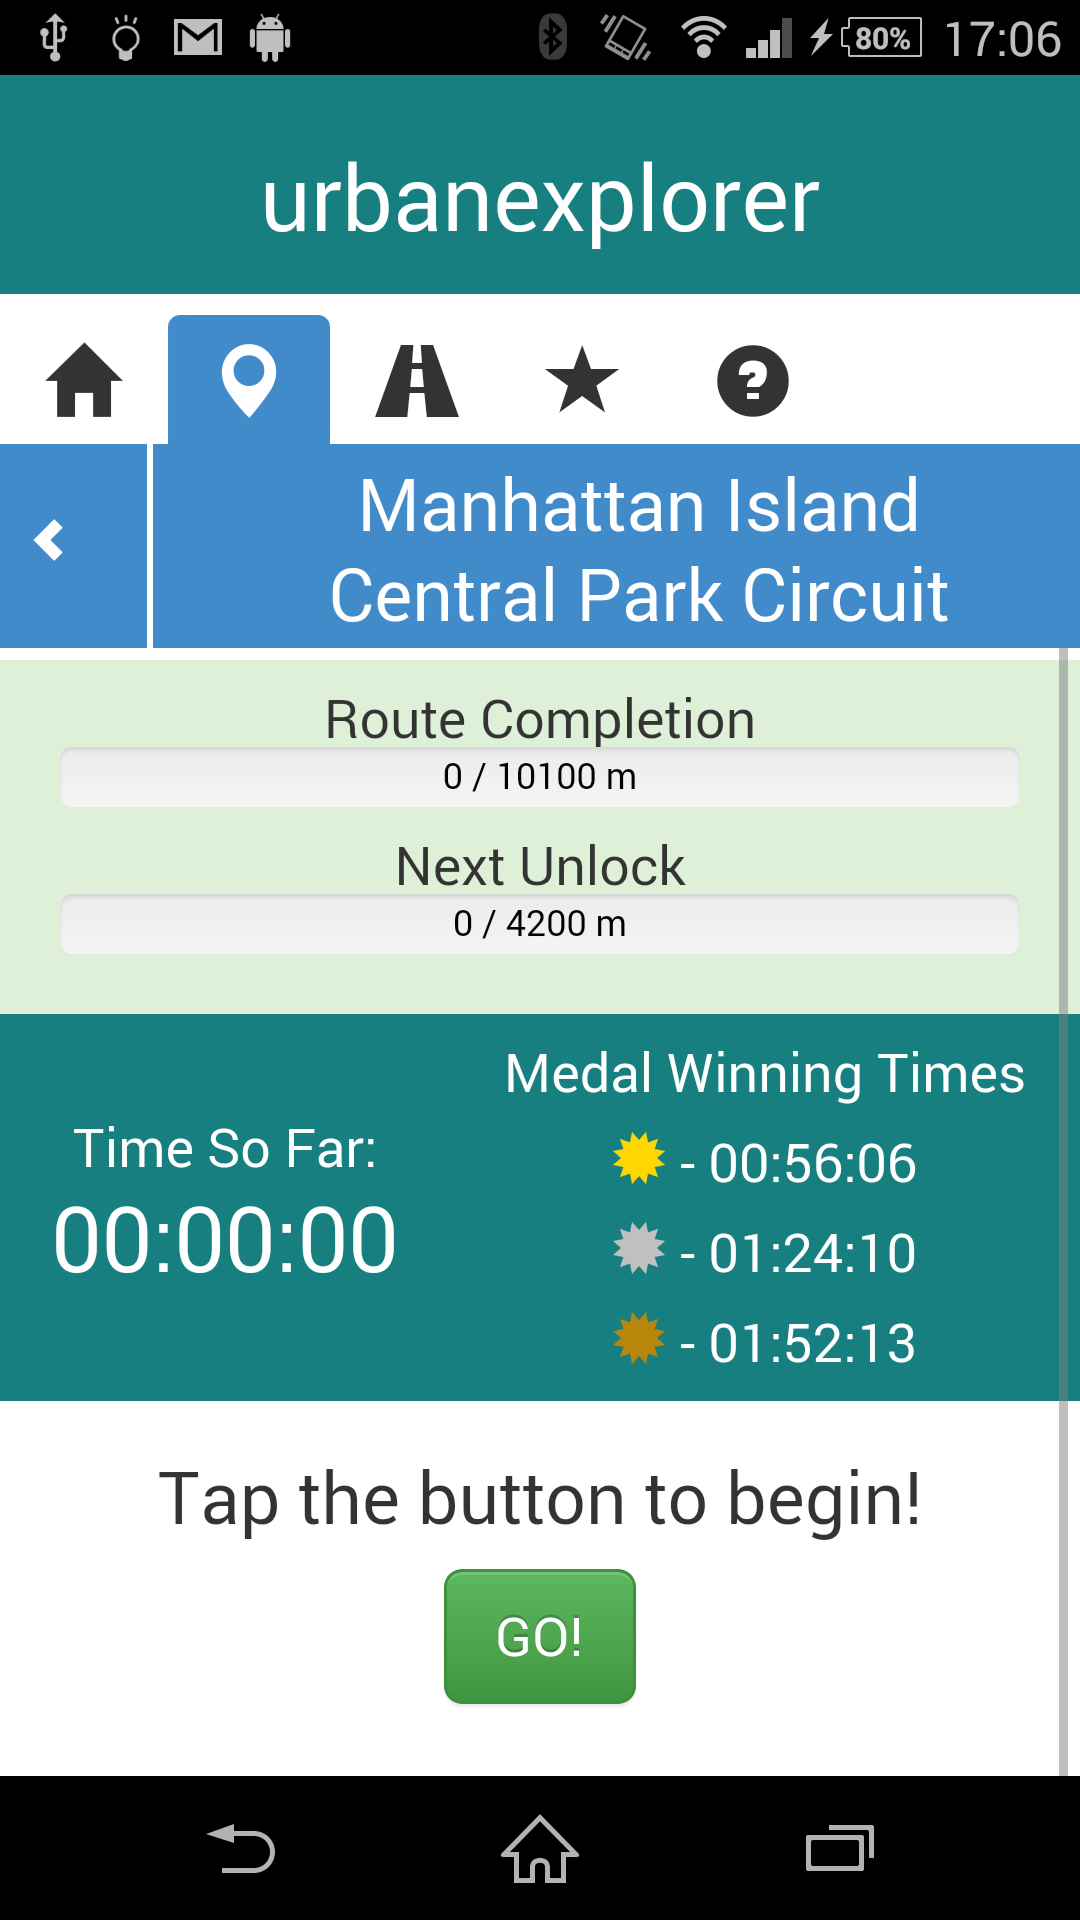
\includegraphics[width=\textwidth]{images/route.png}
    \end{subfigure}
    \hspace{0.02\textwidth}
    \begin{subfigure}[b]{0.3\textwidth}
      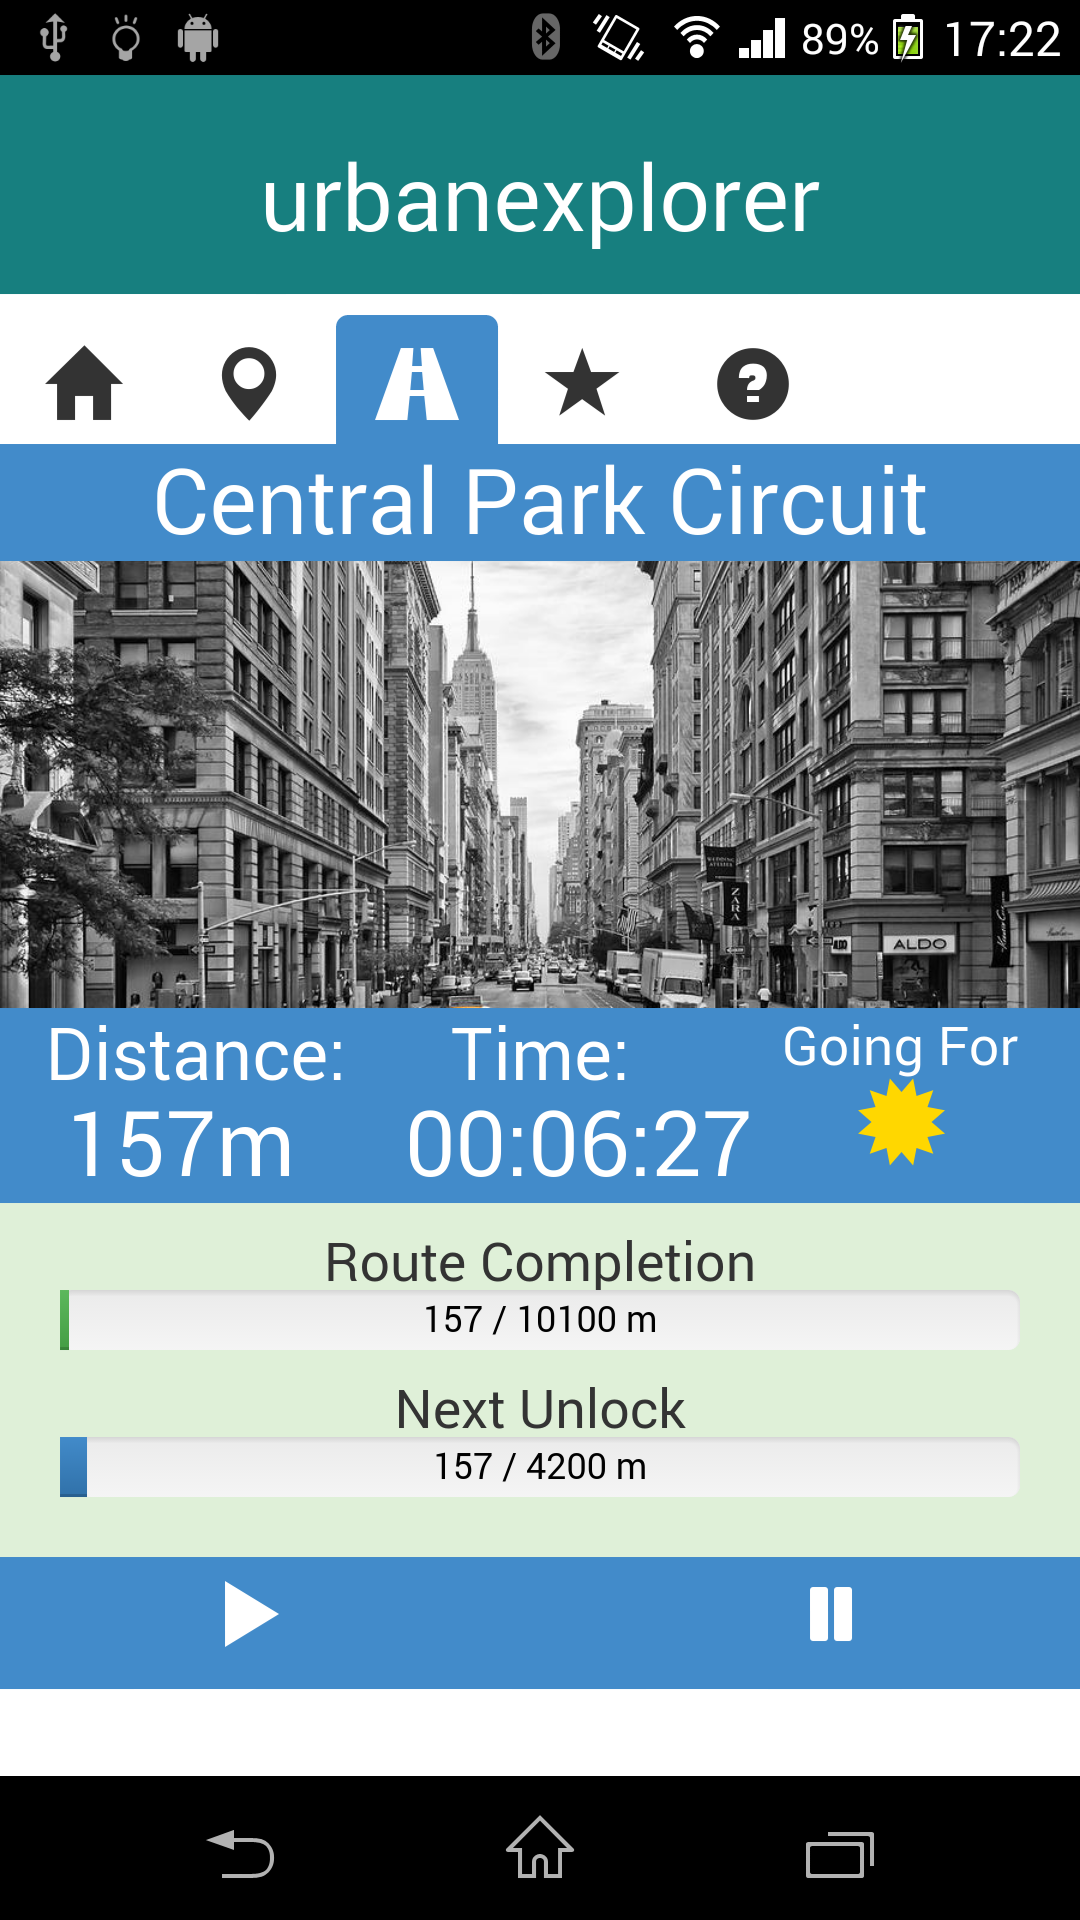
\includegraphics[width=\textwidth]{images/run.png}
    \end{subfigure}
  \end{figure}
\end{frame}

\begin{frame}
  \frametitle{Urban Explorer}
  \begin{itemize}
    \item User picks a route they wish to run along.
    \item User runs outdoors where distance is tracked via GPS.
    \item The distance travelled is added to their chosen route.
    \item May be physically running around Kelvin Park but they are
      running around Central Park inside the app.
    \item Receive a medal for completing the route in a given time.
    \item Unlock pictures as you travel along the route.
  \end{itemize}
  \begin{figure}[h]
    \centering
    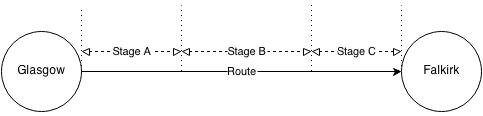
\includegraphics[width=0.8\textwidth]{images/route_breakdown.jpg}
  \end{figure}
\end{frame}

\begin{frame}
  \frametitle{Design Goals}
  Reduce \emph{cost} for the user:
  \begin{enumerate}
    \item Time - Loading time, navigation time
    \item Data - Monetary charges incurred to the user through network
      transfer.
  \end{enumerate}
  
  Make a gamified experience that encourages the user to exercise.
\end{frame}

\begin{frame}
  \frametitle{Platforms}
  \begin{itemize}
    \item PhoneGap (app only released on Android)
    \item AngularJS JavaScript Framework
    \item Twitter Bootstrap CSS3 Framework
    \item Django middleware with built-in ORM
    \item Django-Tastypie for REST API generation
  \end{itemize}
\end{frame}

\begin{frame}
  \frametitle{N-Tier Diagram}
  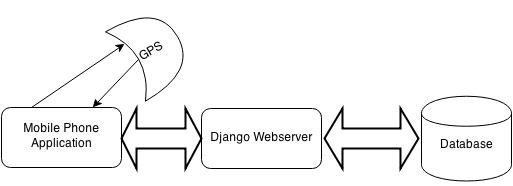
\includegraphics[width=\textwidth]{images/n-tier.jpg}
\end{frame}

\begin{frame}
  \frametitle{Entity Relation Diagram}
  \begin{figure}[h]
    \centering
    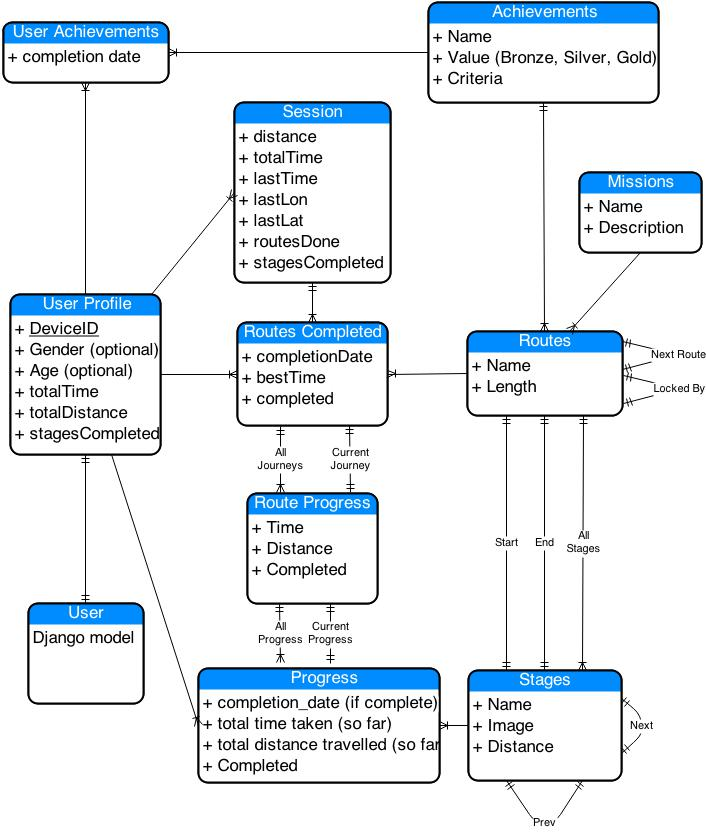
\includegraphics[width=0.6\textwidth]{images/ER_prod.jpg}
  \end{figure}
\end{frame}

\begin{frame}
  \frametitle{Notable Design Decisions}
  \begin{itemize}
    \item Explicit Caching
    \item Promise Based Module Interfaces
    \item Exercise Session Management
    \item Location Management
    \item Distance Verification
  \end{itemize}
\end{frame}

\begin{frame}
  \frametitle{Location Management}
  \begin{itemize}
    \item How often should we request location information?
    \item Location information is costly: 50-200mA. Almost as costly
      as a 3G message.
    \item Chose once a minute based on measuring round-trip-time of
      entire process.
    \item Cul-de-sac effect. Similar to aliasing in signal analysis.  
    \item Can me mitigated by getting location information more
      frequently. 
  \end{itemize}
\end{frame}

\begin{frame}
  \frametitle{Cul-de-sac effect}
  \begin{figure}[h]
    \centering
    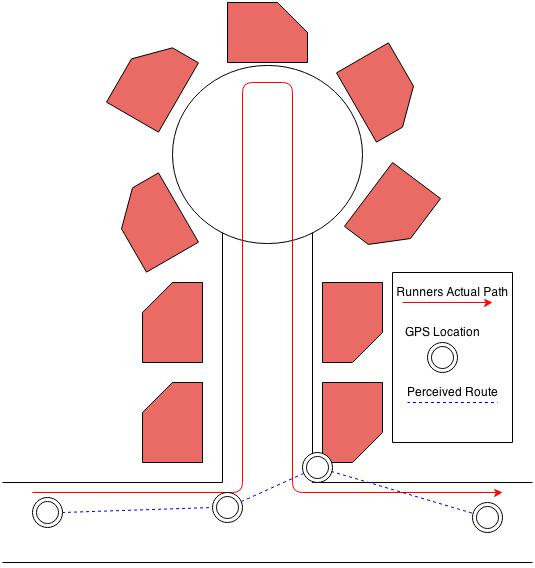
\includegraphics[width=0.65\textwidth]{images/cul-de-sac.jpg}
  \end{figure}
\end{frame}

\begin{frame}
  \frametitle{Distance Verification}
  \begin{itemize}
    \item Haversine Function.
    \item Try to hamper cheating attempts.
    \item Device uploads coordinates to the server where distance is
      calculated. 
    \item Maximum speed that a user can travel is 6$m/s$.
    \item Worst case inaccuracy due to the ``Cul-de-sac'' effect is
      360$m$ when requesting location information at one minute intervals.
  \end{itemize}
\end{frame}

\begin{frame}
  \frametitle{Evaluation}
  \begin{itemize}
    \item Two main design and evaluation iterations.
    \item Initial design was distributed to a small group.
    \item Final design was openly distributed. Over 40 total downloads
      and 9 actual engagements.
    \item From these 9 users, three completed a route and two were
      awarded medals.
    \item Survey was circulated asking for feedback about the platform
      and gamification. Received 8 responses.
  \end{itemize}
\end{frame}

\begin{frame}
  \frametitle{Evaluation}
  \begin{table}[h]
    \centering
    \small
    \begin{tabular}{| c | c | c | c | c | c | c |} \hline
      % Headings
      ID & 
      \multicolumn{1}{p{1.7cm}|}{\centering Time \\ (hh:mm:ss)} & 
      \multicolumn{1}{p{1.3cm}|}{\centering Distance \\ (m)} &
      \multicolumn{1}{p{1.0cm}|}{\centering Stages} & 
      \multicolumn{1}{p{1.0cm}|}{\centering Routes} &
      \multicolumn{1}{p{1.5cm}|}{\centering Exercise \\ Sessions} &
      Medals \\\hline
      %% Content
      e4...ee & 09:40:46 & 20027 & 11 & 4 & 1 & - \\\hline
      94...70 & 03:17:51 & 11805 & 5 & 1 & 2 & Silver \\\hline
      5e...8f & 02:16:10 & 4038 & 0 & 0 & 1 & - \\\hline
      2a...42 & 01:54:42 & 15141 & 39 & 2 & 3 & Gold \\\hline
      56...b4 & 00:02:02 & 2 & 0 & 0 & 2 & - \\\hline
      7e...69 & 00:01:21 & 74 & 0 & 0 & 2 & - \\\hline
      d3...ba & 00:01:10 & 103 & 0 & 0 & 1 & - \\\hline
      36...da & 00:00:20 & 23 & 0 & 0 & 2 & - \\\hline
      46...05 & 00:00:01 & 0 & 0 & 0 & 1 & - \\\hline
    \end{tabular}
    \caption{Active users of ``Urban Explorer'' ranked by time invested.}
    \label{table:usage}
  \end{table}
\end{frame}

\begin{frame}
  \frametitle{Evaluation}
  Points from survey responses:
  \begin{itemize}
    \item Responses indicated a positive experience with the app.
    \item Medals were rated very encouraging (4.14/5 avg.)
    \item Picture unlocks were less encouraging (3.43 avg.)
    \item However viewing these pictures as you exercise was met with
      a better response (3.57 avg.)
    \item Standard statistics are still important to users for
      encouragement (3.71 avg.)
  \end{itemize}
\end{frame}

\begin{frame}
  \frametitle{Evaluation}
  Points from survey responses:
  \begin{itemize}
    \item Responses indicated dissatisfaction with how often the
      distance was updated (2.83 avg.) and users were not convinced
      that the distance reported was accurate (3/5 avg.).
    \item Goals were clear (4.33/5 avg.) and encouraging (3.5/5 avg.).
  \end{itemize}
\end{frame}

\begin{frame}
  \frametitle{Future Work}
  Technology:
  \begin{itemize}
    \item Implement as a native Android app, do not use PhoneGap for
      production quality applications.
    \item Determine the best solution to mitigate the ``Cul-de-sac''
      effect while preserving battery life.
    \item Google Play Location Services for location information.
  \end{itemize}
\end{frame}

\begin{frame}
  \frametitle{Future Work}
  Gamification:
  \begin{itemize}
    \item Better onboarding techniques required
    \item Emphasise short-term goals 
    \item Reminders to exercise
    \item Local Leaderboards of achievement
    \item Social interaction
      \begin{itemize}
        \item Create a team of peers to work towards longer goals
        \item Global routes that every player contributes too.
      \end{itemize}
    \item Expand story to include a \emph{discovery} element.
  \end{itemize}
\end{frame}

\begin{frame}
  \frametitle{Walk Around The World}
  \begin{center}
    Thank You to Leif Azzopardi and David Maxwell.
    \\
    Questions?
  \end{center}
\end{frame}

\end{document}
